\section{Resultados}

% LES COPIO LO QUE TENIA EN EL CUADERNO:
% 	Delays en distintos momentos del dia? 
%	Se congestionan los enlaces en horas pico? (ver cuales son las horas pico en cada pais del enlace). 
%	Se utilizan los enlaces si voy a otras paginas cercanas a las que probamos? 
%	Cambian las rutas que se toman a una misma pagina? 
%	Ver tiempos de encolamiento (hacer algun tipo de analisis sobre esto supongo)

Los datos de los siguientes graficos se midieron utilizando el Traceroute implementado por nosotros. El metodo de medicion fue el siguiente:

***** ACA NO ESTOY SEGURO DE COMO VICKY HIZO LAS MEDICIONES.. POR FAVOR COMPLETAR!! ****

En las figuras \ref{fig:mapa_fin} y \ref{fig:mapa_ing} se muestran una localizacion aproximada de los enlaces transoceanicos encontrados.\\

El primero es un enlace de Estados Unidos (Florida segun IP2Location, Colorado segun IPLigence), a ``Europa'' (segun \url{http://www.geoiptool.com/es/} y \url{www.ipaddresslabs.com})\\

\begin{itemize}
 \item IP del lado de America: 67.17.106.162
 \item IP del lado de Europa: 213.248.76.189\\
\end{itemize}
    
Como ip final (reply) se utilizo el host \url{www.helsinki.fi} (IP: 128.214.222.4). Este host se encuentra en Finlandia


El segundo es un enlace de Estados Unidos (Colorado segun IPligence) a Alemania (segun IPligence)

\begin{itemize}
 \item IP del lado de America: 67.16.139.18
 \item IP del lado de Europa: 141.136.107.37\\
\end{itemize}

El host final del Traceroute fue un host de inglaterra: \url{www.ox.ac.uk} (IP: 163.1.60.42)

\begin{figure}[H]
  \centering
    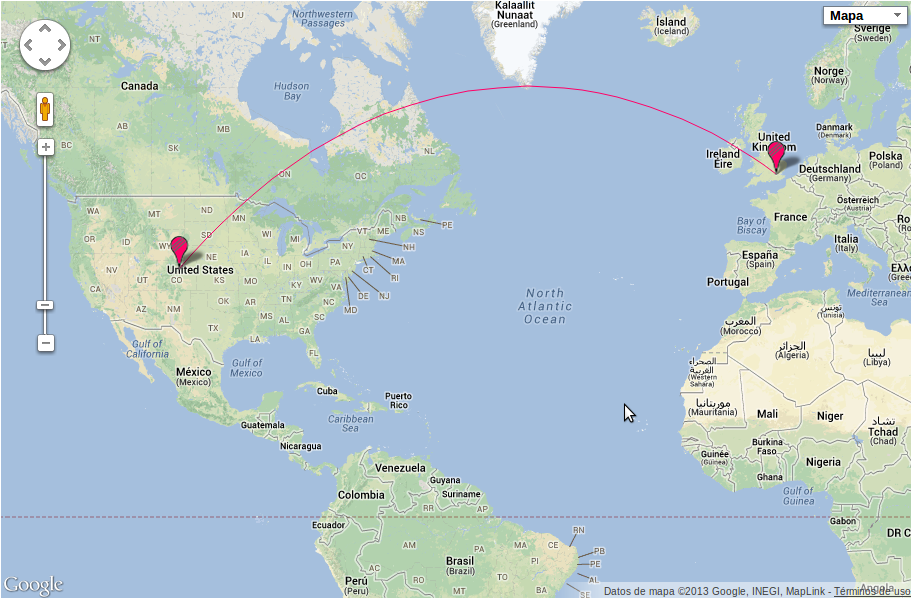
\includegraphics[width=0.9\textwidth]{imgs/finlandia_enlace_1.png}
    \caption{Mapa con la ubicacion aproximada del enlace tomado hacia el host \url{www.helsinki.fi} (Finlandia)}
    \label{fig:mapa_fin}
\end{figure}


\begin{figure}[H]
  \centering
    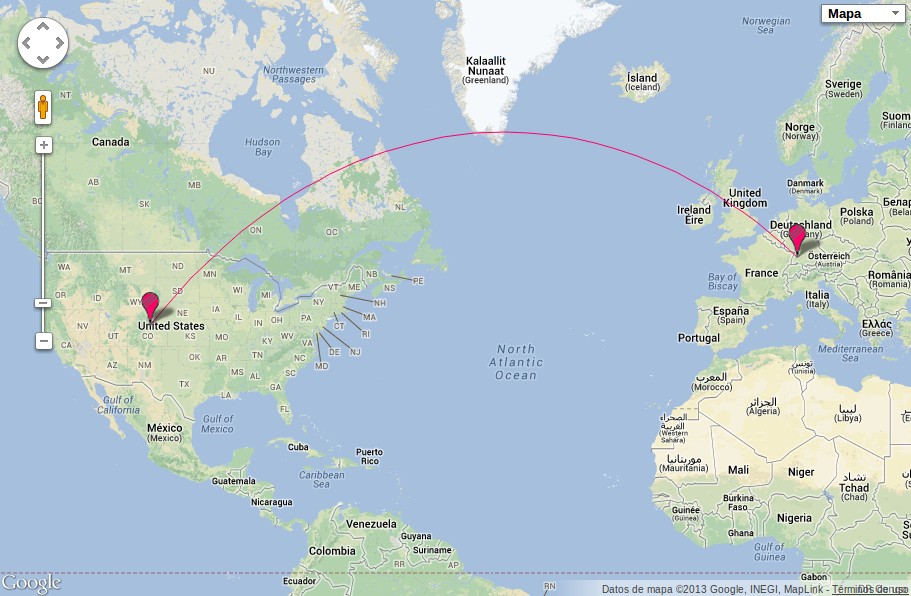
\includegraphics[width=0.9\textwidth]{imgs/inglaterra_enlace_1.png}
    \caption{Mapa con la ubicacion aproximada del enlace tomado hacia el host \url{www.ox.ac.uk} (Inglaterra)}
    \label{fig:mapa_ing}
\end{figure}


\begin{figure}[H]
  \centering
    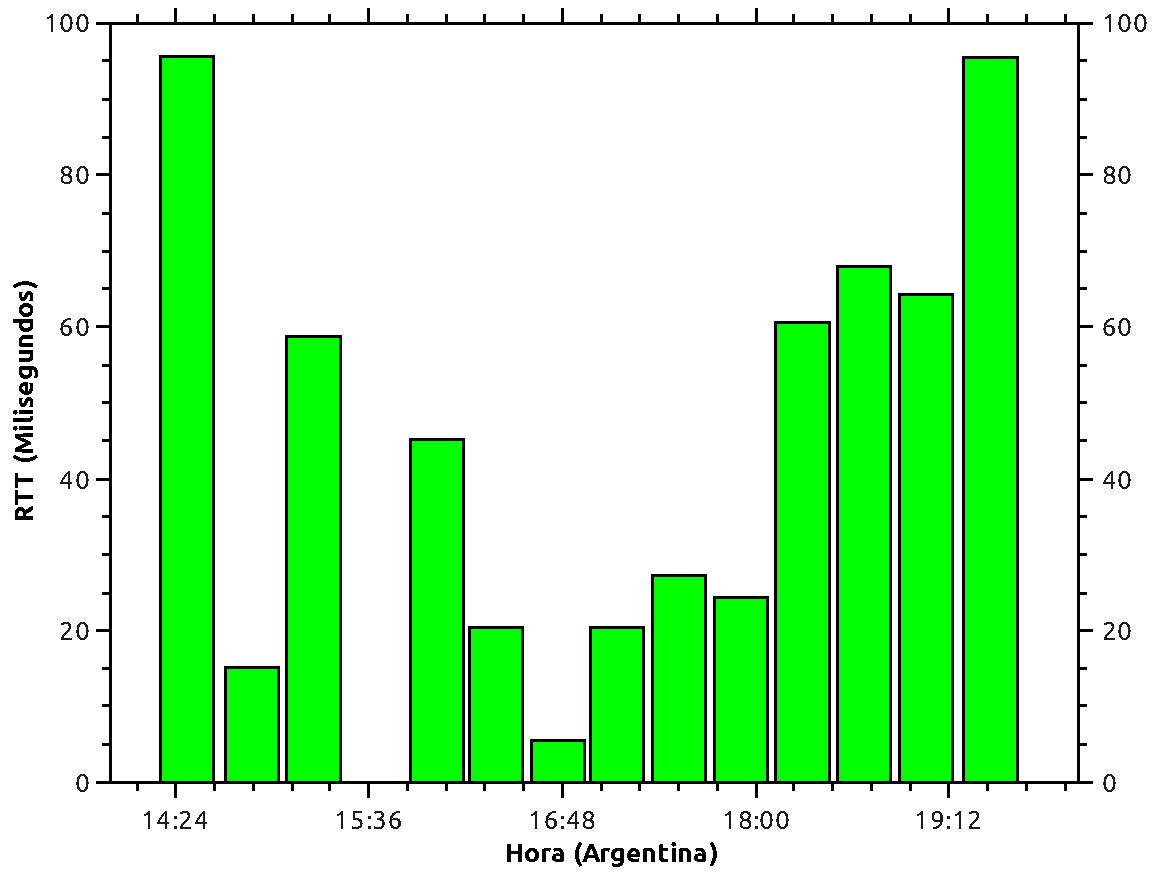
\includegraphics[width=0.9\textwidth]{graficos/rtts_dia_finlandia.pdf}
    \caption{RTTs medidos a lo largo del dia en un enlace de EEUU a finlandia}
    \label{fig:rtts_fin}
\end{figure}

%EEUU : -3
%FINLANDIA: +4

En la figura \ref{fig:rtts_fin} se puede ver como los RTT varian constantemnte durante todo el dia, pricipalmente porque estos enlaces no solo son utilizados por estados unidos, sino por varios host ubicados en todo el continente americano. Esto quiere decir que, cuando en un pais esta en una hora donde se espera haber mucho trafico, en otro pais puede ser, por ejemplo, las 4hs AM, por lo que no es esperable que se congestione la red. 

De todas formas, pese a esto se pueden ver a grandes rasgos como a las 16hs de Argentina, el cual equivale a un rango de entre las 11hs y las 16hs de todo el continente americano, este enlace parece estar mucho menos congestionado que entre las 16 y las 20hs. 

%%% Aca hay q pulirlo.. esta medio chori.. le falta poder de sintesis :P, capas meter alguna tabla con zonas horarias.. y sacar alguna conclusion de trafico segun momento del dia..


\begin{figure}[H]
  \centering
    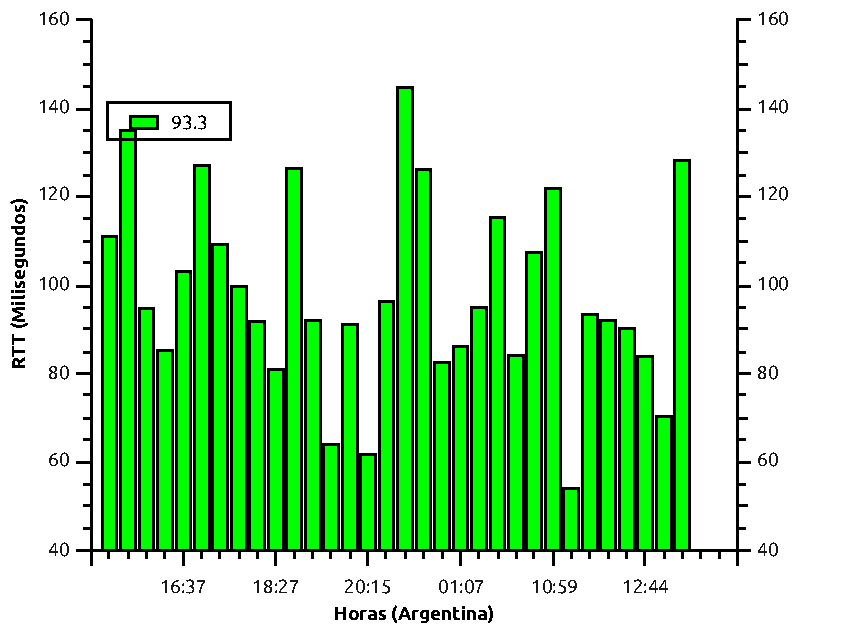
\includegraphics[width=0.9\textwidth]{graficos/rtts_dia_inglaterra.pdf}
    \caption{RTTs medidos a lo largo del dia en un enlace de EEUU a finlandia}
    \label{fig:rtts_ing}
\end{figure}